% --- [ Decompilation Phases ] -------------------------------------------------

\subsection{Decompilation Phases}
\label{sec:decompilation_phases}

A core principle utilized in decompilers is the separation of concern through the use of abstractions, and extensive work involves translating into and breaking out of various abstraction layers. In general, a decompiler is composed of distinct phases which parses, analyses or transforms the input. These phases are conceptually grouped into three modules to separate concerns regarding source machine language and target programming language. Firstly, the front-end module parses executable files and translates their platform dependent assembly into a platform independent intermediate representation (IR). Secondly, the middle-end module performs a set of decompilation passes to lift the IR, from a low-level to a high-level representation, by reconstructing high-level control structures and expressions. Lastly, the back-end module translates the high-level IR to a specific target programming language \cite{reverse_comp}. Figure \ref{fig:modules_overview} gives an overview of the decompilation modules and visualizes their relationship.

\begin{figure}[htbp]
	\begin{center}
		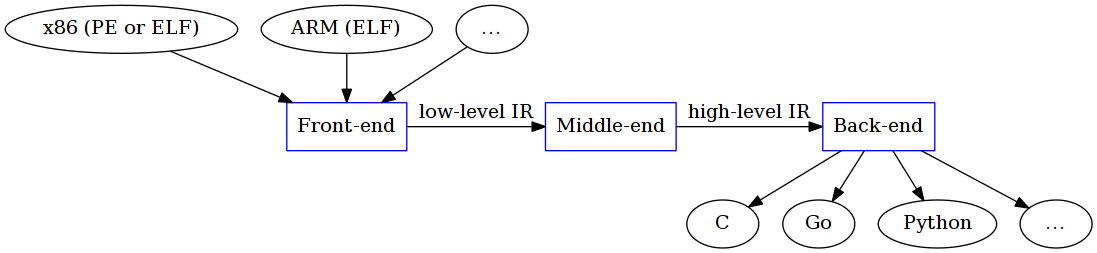
\includegraphics[width=\textwidth]{inc/modules_overview.png}
		\caption{Firstly, the front-end module accepts several executable file formats (PE, ELF, …) as input and translates their platform dependent assembly (x86, ARM, …) to a low-level IR. Secondly, the middle-end module then lifts the low-level IR to a high-level IR through a set of decompilation passes. Lastly, the backend-module translates the high-level IR into one of several target programming languages (C, Go, Python, …).}
		\label{fig:modules_overview}
	\end{center}
\end{figure}

The remainder of this section describes the distinct decompilation phases, most of which have been outlined by Cristina Cifuentes in her influential paper \textit{``Reverse Compilation Techniques''} \cite{reverse_comp}.
